\chapter{List of primitives }
\label{liste-prim} The turtle is controlled by means of internal commands
called \emph{`primitives'} . The following sections set out these
primitives:
\section{Movement of the turtle; pen and color settings}
These first primitives govern the movement of the turtle.\\
\prim{forward, fd}{n}
 Moves the turtle forward n steps in the direction it is currently facing.\\
\prim{back, bk}{n}
 Moves the turtle backwards n steps in the direction it is currently facing.\\
\prim{right, rt}{n}
 Turns the turtle n degrees towards the right in relation to the direction it is currently facing.\\
\prim{left, lt}{n}
 Turns the turtle n degrees towards the left in relation to the direction it is currently facing.\\
\prim{circle}{R}
 Draws a circle of R radius around the turtle.\\
\prim{arc}{R cap1 cap2}
Draws an arc of R radius around the turtle. This arc is inscribed between the caps cap1 and cap2.\\
\prim{home}{}
 Returns the turtle to its initial position, that is, the co-ordinates {[}0 0{]} with a heading of 0 degrees.\\
\prim{setpos, setposition}{list}
 Moves the turtle to the co-ordinates specified by the two numbers in the list (x specifies the x-axis and y the y-axis)\\
\prim{setx}{x}
 Moves the turtle horizontally to the point x on the x-axis\\
\prim{sety}{y}
 Moves the turtle vertically to the point y on the y-axis\\
\prim{setxy}{x y}
 Identical to setpos {[}x y{]}\\
\prim{setheading, seth}{n}
 Orients the turtle in the specified direction. 0 corresponds to a position facing vertically upwards.  The heading when the turtle is rotated is then based on compass bearings. \\
\prim{label}{arg}
Draw the specified word or list at the turtle's location, and following the direction it is facing.\\
 Eg: \texttt{label [Hello there!]} will write the sentence "Hello there!" wherever the turtle is, and corresponding to its bearing or heading.\\
\prim{dot}{list}
The point defined by the co-ordinates in the list will be highlighted (in the pen colour).\\ \\

This second group sets out the primitives which allow the properties of the turtle to be adjusted. For example, should the turtle be visible on screen? What colour should it draw when it moves? \\
\prim{showturtle, st}{}
 Makes the turtle visible on the screen.\\
\prim{hideturtle, ht}{}
 Makes the turtle invisible on the screen.\\
\prim{clearscreen, cs}{}
 Empties the drawing area.\\
\prim{wash}{}
 Erases the drawing area but leaves the turtle in the same place.\\
\prim{resetall}{}
 Initialize the \xlogo\ interface to standard values.
\begin{itemize}
 \item PenColor: black
 \item ScreenColor:white
 \item Animation mode: disabled 
 \item Text and Graphics Font: Dialog 12 pts
 \item Pen shape: square
 \item Drawing quality: normal
 \item Turtles allowed: 16
 \item Mode trace: disabled
 \item Screen size: 1000x1000
\end{itemize}
and empties the drawing area.\\
\prim{pendown, pd}{}
 The turtle will draw a line when it moves.\\
\prim{penup, pu}{}
 The turtle will not draw a line when it moves.\\
\prim{penerase, pe}{}
 The turtle will rub out any marks that it meets.\\
\prim{penreverse, px}{}
 Lower the pen and put the turtle in inverted mode.\\
\prim{penpaint, ppt}{}
 Lower the pen and put the turtle in classic drawing mode.\\
\prim{setpencolor, setpc}{color}
 Sets the pen color. See p.\pageref{couleurs}.\\
\prim{setscreencolor, setsc}{color}
 Sets the screen color. See p.\pageref{couleurs}.\\
\prim{pos, position}{}
 Gives the current position of the turtle.Eg: \texttt{pos} returns {[}10 -100{]}\\
\prim{x}{}
 Returns the x-coordinate of the turtle position.\\
\prim{y}{}
 Returns the y-coordinate of the turtle position.\\
\prim{z}{}
 Returns the z-coordinate of the turtle position. (Only available in 3D mode)\\
\prim{heading}{}
 Gives the bearing or heading of the turtle (cf \texttt{setheading})  \\
\prim{towards}{list}
The list must contain two numbers representing co-ordinates.  Gives the heading which the turtle must follow to go towards the point defined by the co-ordinates in the list.\\
\prim{distance}{list}
The list must contain two numbers representing co-ordinates.  Gives the number of steps between the current position and the point defined by the co-ordinates in the list.\\
\prim{pencolor, pc}{}
 Gives the current colour of the pen.  This colour is specified by a list [r g b] where r is the red component, b the blue and g the green.  \\
\prim{screencolor, sc}{}
 Gives the current colour of the screen (background).  This colour is specified by a list [r g b] where r is the red component, b the blue and g the green.  \\
\prim{window}{}
Window configuration: the turtle can travel outside the drawing area (but of course, it cannot draw there).\\
\prim{wrap}{}
Window configuration: if the turtle leaves the drawing area, it will reappear on the opposite side!\\
\prim{fence}{}
Window configuration: the turtle is confined to the drawing area.  If it is about to go outside, an error message will let you know, and give you the maximum number of steps the turtle can move before the exit point is reached (to within 1 or 2 steps ...).\\
\prim{perspective}{}
Window configuration: the turtle can move through 3d Space. (See Special Section \ref{3D} for this mode). To quit this mode, use one of these primitives \texttt{window}, \texttt{wrap} or \texttt{fence}\\
\prim{findcolor, fc}{list}
Returns the colour of the \textit{list} coordinates pixel. This color is determined by a [r g b] list where r is red, g is green and b is blue. \\
\prim{setpenwidth, setpw}{n}
Defines the thickness of the pen nib in pixels.  The default is 1. The pen has a square or round nib.  (Other shapes will be provided in future versions.)\\
\prim{penwidth, pw}{}
Returns the thickness of the pen nib in pixels.\\
\prim{setPenShape, setps}{0-1}
Set the pen shape.
\begin{itemize}
 \item 0$\to$square.
 \item 1$\to$round.
\end{itemize}
\noindent
\prim{PenShape, ps}{}
Returns the pen shape.
\begin{itemize}
 \item 0$\to$square.
 \item 1$\to$round.
\end{itemize}
\noindent
\prim{setDrawingQuality, setdq}{0-1-2}
Set the drawing Quality.
\begin{itemize}
 \item  0$\to$normal.
 \item  1$\to$high.
 \item  2$\to$low.
\end{itemize}
\noindent
\prim{DrawingQuality, dq}{}
Returns the drawing Quality.
\begin{itemize}
 \item  0$\to$normal.
 \item  1$\to$high.
 \item  2$\to$low.
\end{itemize}
\noindent
\prim{setscreensize}{list}
Set the screen size to the dimension contained in the list. \texttt{setscreensize [1000 1000]}\\
\prim{screensize}{}
Returns the current screen size in a list. \texttt{setscreensize [1000 1000]}\\
\prim{setshape}{n}
You can choose your preferred turtle with the second tab of menu Options-Preferences.... But you can choose your favourite turtle with \texttt{setshape}. The number n goes from 0 to 6. (0 is the triangular shape).\\
\prim{shape}{}
Returns the number that represents the shape of the turtle.\\
\prim{setfontsize, setfs}{n}
When you write on the screen with the primitive \texttt{label}, it's possible to modify the size of the font with \texttt{setfontsize}. The size of the font is 12 by default.\\
\prim{fontsize}{}
Returns the size of the font when you write on the screen with the primitive \texttt{label}.\\
\prim{setfontname, setfn}{n}
Select the font number $n$ when you write on the screen with the primitive \texttt{label}. You can find the link between number and font in Menu$\to$OptionsvPreferences$\to$Tab Font.\\
\prim{setfontjustify}{list}
When you write on the screen with the primitive \texttt{label}, it's possible to specify the text alignment around the turtle. The list contains two integers.
\begin{itemize}
 \item The first integer represents the horizontal alignment.
	\begin{itemize}
 	\item 0: left horizontal alignment.
	\item 1: center horizontal alignment.
	\item 2: right horizontal alignment.
	\end{itemize}
 \item The second integer represents the vertical alignment.
	\begin{itemize}
 	\item 0: bottom vertical alignement.
	\item 1: center vertical alignment.
	\item 2: top vertical alignment.
	\end{itemize}
\end{itemize}
Here are all possible cases:
\texttt{setfontsize 50 label "XLogo}
\begin{center}
 \begin{tabular}{|c|c|c|}
 \hline

\includegraphics[width=3cm]{pics/fap20.png} & 
\includegraphics[width=3cm]{pics/fap10.png} & 
\includegraphics[width=3cm]{pics/fap00.png} \\
\texttt{setfontjustify [2 0]} & \texttt{setfontjustify [1 0]} & \texttt{setfontjustify [0 0]}\\
 \hline

\includegraphics[width=3cm]{pics/fap21.png}& 
\includegraphics[width=3cm]{pics/fap11.png} & 
\includegraphics[width=3cm]{pics/fap01.png} \\
\texttt{setfontjustify [2 1]} & \texttt{setfontjustify [1 1]} & \texttt{setfontjustify [0 1]}\\
 \hline

\includegraphics[width=3cm]{pics/fap22.png}& 
\includegraphics[width=3cm]{pics/fap12.png} & 
\includegraphics[width=3cm]{pics/fap02.png} \\
\texttt{setfontjustify [2 2]} & \texttt{setfontjustify [1 2]} & \texttt{setfontjustify [0 2]}\\
 \hline
\end{tabular}
\end{center}
\hspace{0cm}\\
\prim{fontjustify}{}
Returns a list that represents the text alignment around the turtle when you write on drawing area with the primtive \texttt{label}\\
\prim{fontname}{}
Returns a list with two elements. The first is the number corresponding to the font used when you write on the screen with the primitive \texttt{label}. The last element is a list which contains the name of the font.\\
\prim{setseparation, setsep}{n}
Determines the ratio between the graphic screen and the history zone. The number $n$ must be included between 0 and 1. When $n$ equals 1 the drawing zone uses all the space, when $n$ equals 0, the history zone uses all the window.\\
\prim{separation,sep}{}
Provides the current ratio between the drawing zone and the history zone.\\
\prim{grid}{a b}
Draw a grid. Each square has dimension $a$ and $b$.\\
\prim{stopgrid}{}
Erase grid.\\
\prim{setgridcolor}{color}
Allow the user to choose a custom color for the grid. Eg: \texttt{setgridcolor red}\\
\prim{gridcolor}{}
Returns current grid color.\\
\prim{grid?}{}
Return true if the grid is drawn, else return false.\\
\prim{axis}{n}
Draw horizontal and vertical axis. The distance between two divisions is $n$ steps. \\
\prim{xaxis}{n}
Draw only horizontal axis. The distance between two divisions is $n$ steps.\\
\prim{yaxis}{n}
Draw only vertical axis. The distance between two divisions is $n$ steps.\\
\prim{stopaxis}{}
Erase both axis.\\
\prim{setaxiscolor, sac}{color}
Allow the user to choose a custom color for the axis. Eg: \texttt{setaxiscolor green} \\
\prim{axiscolor}{}
Returns current axis color.\\
\prim{xaxis?}{}
Return true if the horizontal axis is drawn, else return false.\\
\prim{yaxis?}{}
Return true if the vertical axis is drawn, else return false.\\
\prim{setzoom}{a}
Zoom on the drawing screen. In fact, the number \textit{a} represents the scale regarding to the original image size fixed in the preference panel.\\
\prim{zoom}{}
Returns the current zoom scaling.\\
\prim{labellength}{arg}
Returns the length that needs the word or the list to be displayed on the screen with the primitive \texttt{label} using the current font. \\
\prim{zonesize}{}
Returns a list which contains four numbers. These integers are the coordinates of the left upper corner of the drawing zone and the coordinates for the right bottom corner.\\
\prim{message, msg}{list}
 Shows the message in list in a dialog box, the program stops until the user has clicked the button "OK"\\
\subsection{A word on colors}
Colors are defined in \xlogo\ with a list of three numbers \texttt{[r g b]} between 0 and 255. The number \texttt{r} is the red component, \texttt{b} the blue and \texttt{g} the green. Xlogo has 16 predefined colours: you can access with their rgb list, with a number, or with a primitive. look at  this table: \label{couleurs}
\begin{center}
\begin{longtable}{*{4}{|c}|}
\hline
Number & Primitives & [R G B] & Color \\ \endhead
\hline
0& \texttt{black} & [0 0 0] & \index{black}
\begin{minipage}[m]{1.5cm}
\begin{center}
\vspace{0.2cm}

\includegraphics[width=1 cm]{pics/couleur0.png}
\vspace{0.2cm}
\end{center}
\end{minipage}\\
\hline
1 & \texttt{red} & [255 0 0] & \index{red}
\begin{minipage}[m]{1.5cm}
\begin{center}
\vspace{0.2cm}

\includegraphics[width=1 cm]{pics/couleur1.png}
\vspace{0.2cm}
\end{center}
\end{minipage}\\\hline
2 & \texttt{green} & [0 255 0] & \index{green}
\begin{minipage}[m]{1.5cm}
\begin{center}
\vspace{0.2cm}

\includegraphics[width=1 cm]{pics/couleur2.png}
\vspace{0.2cm}
\end{center}
\end{minipage}\\
\hline
3 & \texttt{yellow} & [255 255 0] & \index{yellow}
\begin{minipage}[m]{1.5cm}
\begin{center}
\vspace{0.2cm}

\includegraphics[width=1 cm]{pics/couleur3.png}
\vspace{0.2cm}
\end{center}
\end{minipage}\\
\hline
4 & \texttt{blue} & [0 0 255] & \index{blue}
\begin{minipage}[m]{1.5cm}
\begin{center}
\vspace{0.2cm}

\includegraphics[width=1 cm]{pics/couleur4.png}
\vspace{0.2cm}
\end{center}
\end{minipage}\\
\hline
5 & \texttt{magenta} & [255 0 255] & \index{magenta}
\begin{minipage}[m]{1.5cm}
\begin{center}
\vspace{0.2cm}

\includegraphics[width=1 cm]{pics/couleur5.png}
\vspace{0.2cm}
\end{center}
\end{minipage}\\
\hline
6 & \texttt{cyan} & [0 255 255] & \index{cyan}
\begin{minipage}[m]{1.5cm}
\begin{center}
\vspace{0.2cm}

\includegraphics[width=1 cm]{pics/couleur6.png}
\vspace{0.2cm}
\end{center}
\end{minipage}\\
\hline
7 & \texttt{white} & [255 255 255] & \index{white}
\begin{minipage}[m]{1.5cm}
\begin{center}
\vspace{0.2cm}

\includegraphics[width=1 cm]{pics/couleur7.png}
\vspace{0.2cm}
\end{center}
\end{minipage}\\
\hline
8 & \texttt{gray} & [128 128 128] & \index{gray}
\begin{minipage}[m]{1.5cm}
\begin{center}
\vspace{0.2cm}

\includegraphics[width=1 cm]{pics/couleur8.png}
\vspace{0.2cm}
\end{center}
\end{minipage}\\
\hline
9 & \texttt{lightgray} & [192 192 192] & \index{lightgray}
\begin{minipage}[m]{1.5cm}
\begin{center}
\vspace{0.2cm}

\includegraphics[width=1 cm]{pics/couleur9.png}
\vspace{0.2cm}
\end{center}
\end{minipage}\\
\hline
10 & \texttt{darkred} & [128 0 0] & \index{darkred}
\begin{minipage}[m]{1.5cm}
\begin{center}
\vspace{0.2cm}

\includegraphics[width=1 cm]{pics/couleur10.png}
\vspace{0.2cm}
\end{center}
\end{minipage}\\
\hline
11 & \texttt{darkgreen} & [0 128 0] & \index{darkgreen}
\begin{minipage}[m]{1.5cm}
\begin{center}
\vspace{0.2cm}

\includegraphics[width=1 cm]{pics/couleur11.png}
\vspace{0.2cm}
\end{center}
\end{minipage}\\
\hline
12 & \texttt{darkblue} & [0 0 128] & \index{darkblue}
\begin{minipage}[m]{1.5cm}
\begin{center}
\vspace{0.2cm}

\includegraphics[width=1 cm]{pics/couleur12.png}
\vspace{0.2cm}
\end{center}
\end{minipage}\\
\hline
13 & \texttt{orange} & [255 200 0]& \index{orange}
\begin{minipage}[m]{1.5cm}
\begin{center}
\vspace{0.2cm}

\includegraphics[width=1 cm]{pics/couleur13.png}
\vspace{0.2cm}
\end{center}
\end{minipage}\\
\hline
14 & \texttt{pink} & [255 175 175] & \index{pink}
\begin{minipage}[m]{1.5cm}
\begin{center}
\vspace{0.2cm}

\includegraphics[width=1 cm]{pics/couleur14.png}
\vspace{0.2cm}
\end{center}
\end{minipage}\\
\hline
15 & \texttt{purple} & [128 0 255] & \index{purple}
\begin{minipage}[m]{1.5cm}
\begin{center}
\vspace{0.2cm}

\includegraphics[width=1 cm]{pics/couleur15.png}
\vspace{0.2cm}
\end{center}
\end{minipage}\\
\hline
16 & \texttt{brown} & [153 102 0] & \index{brown}
\begin{minipage}[m]{1.5cm}
\begin{center}
\vspace{0.2cm}

\includegraphics[width=1 cm]{pics/couleur16.png}
\vspace{0.2cm}
\end{center}
\end{minipage}\\
\hline
\end{longtable} 
\end{center}
\begin{verbatim}

# These three instructions are the same
setsc orange
setsc 13
setsc [255 200 0]
\end{verbatim}
\subsection{Animation Mode}
There are two primitives which allow execution of commands witout the turtle displaying them: \texttt{animation} and \texttt{stopanimation}\\
\prim{anim, animation}{}
You go into animation mode. The turtle does not draw on the screen anymore but follows the stored line. To update the drawing on the screen, use the primitive \texttt{repaint}. It is very useful to create an animation or to draw a line faster.\\
\prim{stopanim, stopanimation}{}
Animation mode is finished: you switch back to classical mode. You can see the turtle's moves on screen.\\
\prim{repaint}{}
In animation mode, updates the screen: the image on the drawing area is updated.\\ \\
To identify animation mode, a camera icon appears in the history window. If you click on the icon, the animation mode will stop. It's equivalent to the primitive \texttt{stopanimation}.
\begin{center}
   
\includegraphics[scale=2.5]{pics/animation.png}
\end{center} 

\subsection{Writing in the text area with the primitive \texttt{print} or \texttt{write}}

This table sets out the primitives which allow the properties of the text area to be adjusted. Primitive that control the color and the size of the history area, are available only for the primitives \texttt{print} or \texttt{write}\\
\prim{cleartext, ct}{}
Empties the area containing the command and comment history.\\
\prim{pr, print}{arg}
Shows the argument specified in the history zone.
\begin{verbatim}
print "abcd --------> abcd
pr [1 2 3 4] ----> 1 2 3 4
pr 4 ------------> 4
\end{verbatim}
\noindent \prim{write}{arg1}
The same as for the \texttt{print} primitive but doesn't go back to the start of the line.\\
 \prim{setTextSize, setTS}{n}
 Define the size of the font in the command history. Only valid with the primtive \texttt{print}\\
\prim{textsize, ts}{}
 Returns the size of the font with primitive \texttt{print}.\\
\prim{setTextColor, setTC}{color}
Define the color of the font in command history. Valid only with the primitive \index{print, pr}. See p.\pageref{couleurs}.\\
\prim{TextColor, tc}{}
 Returns the color of the font with the primitive \texttt{print} in the command history.\\
\prim{setTextName, setTN}{n}
Select the font number n when you write on the the command history with the primitive \texttt{print}. You can find the link between number and font in Menu$\to$Options$\to$Preferences$\to$Tab Font.\\
\prim{TextName, tn}{}
Returns a list with two elements. The first is the number corresponding to the font used when you write on the command history with the primitive \texttt{print}. The last element is a list which contains the name of the font.\\
\prim{setstyle, setsty}{arg}
Set the format of the text in the text area. You can choose between seven styles: \texttt{none, bold, italic, strike, underline, superscript, subscript}. If you want several styles together, write them in a list.\\
A few examples for formatting text:\\ \\
\texttt{setstyle [bold underline] print "hello}\\
\textbf{\underline{hello}}\\
\texttt{ssty "strike write [strike] ssty "italic write "\textbackslash\ x ssty "superscript print 2}\\
\sout{strike} $x^2$\\
\prim{sty, style}{}
Returns a list which contains the differents styles used for the primitive \texttt{print}.
\section{Turtle and 3D} \label{3D}
>From version 0.9.92, our turtle can leave its plane and move into 3D space. To switch to this mode, we use the primitive \texttt{perspective}. Welcome to a 3D world!
\subsection{The perspective projection}
To represent a 3D space on a 2D plane, \xlogo\ uses a projection perspective. A camera looks at the 3D scene, where the image from the projection screen is displaying. Here is a little scheme to explain this: 
\begin{center}
\includegraphics*[scale=0.6]{pics/perspective.png}
\end{center}
Some primitives allow us to set the camera position. The screen projection is half the distance from the camera.
\subsection{Understanding orientation in a 3D World}
In a 2D plane, the turtle's orientation was only defined by its heading. In a 3D world, the turtle's orientation is given by 3 angles:
\begin{itemize}
\item Roll: The turtle's angle around axis $(Oy)$
\item Pitch: The turtle's angle around axis $(Ox)$
\item Heading: The turtle's angle around axis $(Oz)$ 
\end{itemize}
In fact, to move itself in the 3D World, the turtle is very similar to an aircraft. Here is a little illustration which represents these 3 values:\\
\begin{minipage}{5.8cm}
\begin{center}
\includegraphics*[scale=0.3]{pics/plane-roll.png}
\textbf{Roll}
\end{center}
\end{minipage}
\begin{minipage}{5.5cm}
\begin{center}
\includegraphics*[scale=0.35]{pics/plane-pitch.png}
\textbf{Pitch}
\end{center}
\end{minipage}
\begin{minipage}{5.5cm}
\begin{center}
\includegraphics*[scale=0.3]{pics/plane-heading.png}
\textbf{Heading}
\end{center}
\end{minipage}\\ \\
It seems quite complex at first, but you will see that a lot of things stay very similar to moving in a 2D plane. Here are the basic primitives for moving in the 3D world:\\
\prim{forward, fd, back, bk}{n}
Same behaviour as in 2D plane.\\
\prim{right, rt, left, lt}{n}
Same behaviour as in 2D plane.\\
\prim{rr, rightroll}{n}
The turtle turns $n$ degrees to the right around its longitudinal axis.\\
\prim{lr, leftroll}{n}
The turtle turns $n$ degrees to the left around its longitudinal axis. \\
\prim{up, uppitch}{n}
The turtle goes $n$ degrees up around its transversal axis.\\
\prim{down, downpitch}{n}
The turtle goes $n$ degrees down around its transversal axis.\\ \\
In the 2D plane, when we want to draw a square of side 200 steps, we write:
\begin{verbatim}
repeat 4[fd 200 rt 90] 
\end{verbatim}
These instructions are still available in the 3D world, where the square is drawn in perspective mode. If the turtle goes down $90$ degrees, we can draw another square and we obtain: \\
\begin{minipage}{7cm}
\begin{verbatim}
cs
repeat 4[fd 200 rt 90]
down 90
repeat 4[fd 200 rt 90]
\end{verbatim}
\end{minipage}
\begin{minipage}{10cm}
\begin{center}
\includegraphics*[scale=0.4]{pics/perspective1.png}
\end{center}
\end{minipage}
\\
You just have to try some examples to understand these orientations and become an expert!\\
You must understand that the 3 rotation primitives are linked together, for example try this:\\ \\
\begin{minipage}{7cm}
\begin{verbatim}
cs
leftroll 90 up 90 rightroll 90
\end{verbatim}
\end{minipage}
\hspace{3cm}
\begin{minipage}{7cm}
\begin{center}
The turtles movement is equivalent to \texttt{left~90} (You can try with your hand simulating the turtle if you don't understand)
\end{center}
\end{minipage}
\subsection{Primitives available in 2D mode and 3D mode}
The following primitives are available in 2D plane or in 3D world. The only difference is the arguments received by the primitives. For example, the primitive \texttt{setpos} or \texttt{setposition} is still waiting for a list as an argument but now, the list must contain three numbers $(x;y;z)$ which represent the three point coordinates. Here are all those primitives:\\ \\

\begin{center}
\begin{tabular}{|cccc|}
\hline
\texttt{circle}&
\texttt{arc}&
\texttt{home}&
\texttt{towards}\\
\hline
\texttt{distance}&
\texttt{setpos, setposition}&
\texttt{setx}&
\texttt{sety}\\
\hline
\texttt{setheading}&
\texttt{label}&
\texttt{labellength}&
\texttt{dot}\\
\hline
\texttt{pos, position}&
\texttt{heading} & &\\
\hline
\end{tabular} \\ \vspace{0.5cm}
\end{center}
\textbf{Primitives only available in 3D mode}\\ \\
\prim{setxyz}{x y z} 
This primitive moves the turtle to the chosen point. This primitive is waiting for three arguments representing the point's coordinates. \texttt{setxyz} is very similar to \texttt{setpos} but the coordinates are not written into a list. \\
Example, \texttt{setxyz -100 200 50}: move the turtle to the point $x=-100;y=200;z=50$\\
\prim{setz}{z}
This primitive moves the turtle to the point with the valid value $z$. \texttt{setz} is waiting for one number as an argument. This primitive is comparable to \texttt{setx} or \texttt{sety}. \\
\prim{setorientation}{list}
Set the turtle's orientation. This primitive waits for a list which contains 3 numbers, the roll, the pitch and the heading.\\
Example, \texttt{setorientation [100 0 58]}: the turtle has roll: 100 degrees, pitch: 0 degree and heading: 58 degrees.\\
\prim{orientation}{}
Returns the turtle's orientation in a list which contains: \texttt{[~roll~pitch~heading~]}. Note the number order, if for example, the orientation value is \texttt{[100 20 90]}, this means that if you want the same orientation starting from the origin position (after a \texttt{clearscreen} instruction), you'll have to write the following sequence:
\begin{center}
\texttt{ rightroll 100 up 20 right 90}
\end{center}
If you inverse the instruction's order, you don't obtain the valid orientation!\\
\prim{setroll}{n} 
The turtle turns around its longitudinal axis to the chosen roll angle.\\
\prim{roll}{}
 Returns the current roll value.\\
\prim{setpitch}{n}
The turtle turns around its transversal axis to the chosen pitch angle.\\
\prim{pitch}{}
Returns the current pitch value.
\subsection{3D Viewer}
A 3D Viewer is included in XLogo, it allows you to visualize your drawing in 3D. This module uses the JAVA3D library, so it's necessary to have java3D fully installed.\\ \\
Here are the rules to use the 3D Viewer:\\
When we create a geometric figure on the drawing area, we have to indicate to the 3D Viewer which shapes we want to record for future visualization. It's possible to record polygons (surfaces), lines, points or text. To use this feature, here are the primitives:\\ \\
\prim{polystart}{}
The following turtle's moves are saved to create a polygon. \\
\prim{polyend}{}
Since the last \texttt{polystart} call, the turtle has gone through several vertices. This new polygon is recorded, its color is defined by all vertices color. This primitive finalizes the polygon. \\
\prim{linestart}{}
The following turtle's moves are saved to create a strip line. \\
\prim{lineend}{}
Since the last \texttt{linestart} call, the turtle has gone through several vertices. This new line is recorded, its color is defined by all vertices color. This primitive finalizes the strip line. \\
\prim{pointstart}{} 
The following turtle's moves are saved to create a point set. \\
\prim{pointend}{}
This primitive finalizes the point set.\\
\prim{textstart}{}
Each time the user displays text on the drawing area with the primitive \texttt{label}, it will be recorded and then displayed by the 3D Viewer.\\
\prim{textend}{}
End of text recording.\\
\prim{view3d polyview}{}
Launch the 3D viewer, all recorded objects are drawn on this new window. You have control of the camera scene:
\begin{itemize}
\item You can rotate the scene by clicking on the mouse's left button.
\item You can translate the scene by clicking on the mouse's right button.
\item You can zoom the scene with the mouse's wheel button.
\end{itemize}
\subsection{Drawing a cube}
\noindent All faces are 400 steps square. Here is the program:
\begin{verbatim}
to square
# we record the vertice square
polystart repeat 4[forward 400 right 90] polyend
end

to simpleCube
# yellow cube 
clearscreen perspective setpencolor yellow
# lateral faces
repeat 4[square penup right 90 forward 400 left 90 rightroll 90 pendown]
# bottom face 
downpitch 90 square uppitch 90
# upper face
forward 400 downpitch 90 square
# visualization
view3d
end
\end{verbatim}
We launch with the command: \texttt{simpleCube}:
\begin{center}
\includegraphics*[scale=0.4]{pics/3dCube1.png}
\end{center}
When we replace in the procedure \texttt{square}, \texttt{polystart} with \texttt{linestart} and \texttt{polyend} with \texttt{lineend}
\begin{center}
\includegraphics*[scale=0.4]{pics/3dCube2.png}
\end{center}
If we had used \texttt{pointstart} and \texttt{pointend} instead of \texttt{linestart} and \texttt{lineend}, we would see on screen only the eight cube vertices. These primitives are very useful to display the point set in 3D Space.
\subsection{Lighting the scene}
You can specify four lights in your 3D scene. By default, the main 3D scene has only two ponctual lights enabled. Click on one of the 4 button lights in the 3D modeler, and this dialog box appears:
\begin{center}
 \includegraphics*[scale=0.6]{pics/CaptureLight.png}
\end{center}
Several light type are available:
\begin{itemize}
\item Ambient light: uniform light, you just have to specify its color.
\item Unidirectional light: diffuses according to a constant direction. It's the same case as a ponctual light when the source is very very far from the observer. For example, the case of sun.
\item Ponctual light: This light has a specified position. This light is similar to a headlight.
\item Spot Light: it is a ponctual light but the light is only displayed in a light cone. You have to specify a value angle for this cone.
\end{itemize}
The best thing is to play with those lights to understand how they work!
\subsection{Fog effect}
You can add a fog effect on the main 3d scene. Click on the cloud button in the 3D scene and this dialog box appears.
\begin{center}
 \includegraphics*[scale=0.6]{pics/CaptureFog.png}
\end{center}
Two fogs are available:
\begin{itemize}
 \item Progressive fog: this fog's opactity is progressive. You have to specify two parameters:
	\begin{itemize}
 	\item The distance from which fog begins.
 	\item The disatnce from which opacity is full\\
	\end{itemize}
\item uniform fog: This fog is uniform on the whole scene. You just have to specify the fog's density.
\end{itemize}
\vspace*{0.2cm}
Example with a progressive fog:
\begin{center}
 \includegraphics*[scale=0.4]{pics/example-fog.png}
\end{center}

\section{Arithmetical and logical operations}
This is a list of number-related commands:\\ \\
\prim{sum}{x y}
 Adds the two numbers $x$ and $y$, and returns the result\\
 Eg: \texttt{sum} \ 40 60 returns 100\\
\prim{difference}{x y}
 Returns $x-y$.\\
 Eg: \texttt{difference} \ 100 20 returns 80\\
\prim{minus}{x}
 Returns the negative of $x$. \\
Eg: \texttt{minus} \ 5 returns -5. \emph{See the note at the end
of this table.}\\
\prim{product}{x y}
 Returns the result of multiplying $x$ by $y$.\\
\prim{div, divide}{x y}
 Returns the result of dividing $x$ by $y$\\
 \texttt{div} \ 3 6 returns 0.5\\
\prim{quotient}{x y}
Returns quotient $x$ by $y$\\
 \texttt{quotient} \ 15 6 returns 2\\
\prim{rem, remainder}{x y}
 Returns the remainder after dividing $x$ by $y$.\\
\prim{mod modulo}{x y}
 Returns $x$ modulo $y$. 
\begin{center}
 $\begin{array}{|c|c|c|c|}
 \hline
x & y & \textrm{\texttt{remainder x y}} & \textrm{\texttt{modulo x y}} \\
\hline
14 & 5 & 4& 4\\
\hline
-14 & 5 &-4 & 1\\
\hline
14 & -5 & 4 & -1\\
\hline
-14 & -5 & -4 & -4 \\
\hline
\end{array}
$
\end{center}
This table shows the différence between \texttt{modulo x y } and \texttt{remainder x y}.\\
\prim{round, rnd}{x}
Returns the nearest whole number to the number $x$.\\
 \texttt{round} \ 6.4 returns 6\\
\prim{integer, int}{x}
Returns the integer part of the number $x$.
 \texttt{integer 8.9} returns 8\\
 \texttt{integer 6.8}  returns 6\\
\prim{power}{x n}
 Returns $x$ raised to the power of $n$.\\
 \texttt{power} \ 3 2 returns 9\\
\prim{squareroot, sqrt}{x}
Returns the square root.\\
\prim{log}{x}
 Returns the logarithm of $x$.\\
\prim{exp}{x}
 Returns the exponential of $x$.\\
\prim{log10}{x}
 Returns the decimal logarithm of $x$.\\
\prim{sine, sin}{x}
 Returns the sine of $x$. ($x$ is expressed in degrees)\\
\prim{cosine, cos}{x}
Returns the cosine of $x$. ($x$ is expressed in degrees)\\
\prim{tangent, tan}{x}
Returns the tangent of $x$. ($x$ is expressed in degrees)\\
\prim{arccosine, acos}{x}
Returns the angle in range [0-180] which cosine is $x$.\\
\prim{arcsine, asin}{x}
Returns the angle which sine is $x$.\\
\prim{arctangent, atan}{x}
Returns the angle which tangent is $x$.\\
\prim{pi}{}
 Returns the number $\pi$ (3.141592653589793)\\
\prim{random, ran}{n}
Returns a random integer between 0 and $n-1$.  \\
\prim{alea}{}
Returns a random number between 0 and 1.  \\
\prim{absolute, abs}{x}
 Returns the absolute value (its numerical value without regard to its sign) of a number.  \\
\prim{setdigits}{n}
Sets the number of digits, it sets the precision while calculating. Some more informations:\\
\begin{itemize}
 \item By default, 16 digits are allowed.
 \item If $n$ is negative, the default mode is choosen. 
 \item If $n$ is esual to 0, all numbers are rounded to the unit.
\end{itemize}
This primitive is useful when you want to calculate with a high precision. Have a look at the example with number $\pi$ p.\pageref{approx-pi}.\\
\prim{digits}{}
Returns the number of digits allowed while calculating. By default, this value is -1.\\
\emph{Important :} Be careful with those primitives which require two parameters! \\
Eg: \begin{tabular}{cc}
 \texttt{setxy} \ a b &
 If b is negative\\
 For example, &
 \texttt{setxy} \ 200 -10\\
\\
\end{tabular}

The \logo\ interpreter will carry out the operation 200-10 (ie it will
subtract 10 from 200). It will therefore conclude that there is only
one parameter (190) when it requires two, and will generate an error
message. To avoid this type of problem, use the primitive {}``\texttt{minus}''
to specify the negative number - \texttt{setxy} 200 \texttt{minus}
10.\\
This is a list of logical operators:\\
\\
\prim{or}{b1 b2}
Returns true if \textit{b1} or \textit{b2} is true, otherwise returns false\\
\prim{and}{b1 b2}
Returns true if \textit{b1} and \textit{b2} is true, otherwise returns false\\
\prim{not}{b1}
Returns the negation of \textit{b1}.
\begin{itemize}
 \item  If \textit{b1} is true, returns false.
 \item  If \textit{b1} is false, returns true.
\end{itemize}

\section{Operations on lists}
\noindent
\prim{word}{word1 word2}
Concatenates the two words \textit{word1} and \textit{word2}.\\
 Eg: \texttt{pr word} \char`\"{}a 1 returns a1\\
\prim{list}{arg1 arg2}
Returns a list composed of \textit{arg1} and \textit{arg2}.\\
 For example, \texttt{list 3 6} returns {[}3 6{]}.\\
 \texttt{list} \ {}{}``a {}``list returns {[}a list{]}\\
\prim{sentence, se}{arg1 arg2}
Returns a list composed of \textit{arg1} and \textit{arg2}. If \textit{arg1} or \textit{arg2} is a list, then each
element of \textit{arg1} and \textit{arg2} will become an element of the resulting list (square
brackets are deleted).\\
 Eg: \texttt{se} \ {}{[}4 3{]} {}``hello returns {[}4 3 hello{]}\\
 \texttt{se} \ {}{[}how are{]} {}``things returns {[}how are things{]}\\
\prim{fput}{arg1 list2}
 Insert \textit{arg1} in the first slot in \textit{list2}.\\
 Eg : \texttt{fput} \ {}{}``cocoa {[}2{]} returns {[}cocoa 2{]}\\
\prim{lput}{arg1 list2}
 Insert \textit{arg1} in the last slot of \textit{list2}.\\
 Eg: \texttt{lput} \ 5 {[}7 9 5{]} returns {[}7 9 5 5{]}\\
\prim{reverse}{list}
 Reverse the order of elements in \textit{list}.\\
 \texttt{reverse} \ {}{[}1 2 3{]} returns {[}3 2 1{]}\\
\prim{pick}{arg1}
\begin{itemize}
 \item If \textit{arg1} is a word, returns one of the letters of \textit{arg1} at random.
 \item  If \textit{arg1} is a list, returns one of the elements of \textit{arg1} at random.
\end{itemize}
\noindent
\prim{remove}{arg1 list2}
Remove element \textit{arg1} from list \textit{list2} if it occurs there.\\
 Eg: \texttt{remove} \ 2 {[}1 2 3 4 2 6 {]} returns {[}1 3 4 6{]}\\
\prim{item}{n arg2}
\begin{itemize}
 \item If \textit{arg2} is a word, returns the letter numbered $n$ from the word (1 represents the first letter).
 \item  If \textit{arg2} is a list, returns the element numbered $n$ from the list.
\end{itemize}
\noindent
\prim{butlast, bl}{arg1}
\begin{itemize}
 \item If \textit{arg1} is a list, returns the whole list except for its last element.
 \item If \textit{arg1} is a word, returns the word minus its last letter.
\end{itemize}
\noindent
\prim{butfirst, bf}{arg1}
\begin{itemize}
 \item If \textit{arg1} is a list, returns the whole list except for its first element.
 \item If \textit{arg1} is a word, returns the word minus its first letter.
\end{itemize}
\noindent
\prim{last}{arg1}
\begin{itemize}
 \item If \textit{arg1} is a list, returns the last element of the list. 
 \item If \textit{arg1} is a word,returns the last letter of the word.
\end{itemize}
\noindent
\prim{first}{arg1}
\begin{itemize}
 \item If \textit{arg1} is a list, returns the first element of the list. 
 \item If \textit{arg1} is a word,returns the first letter of the word.
\end{itemize}
\noindent
\prim{setitem, replace}{list1 n arg3}
Replace the element number \texttt{n} in the list \texttt{list1}, by the word or the list \texttt{arg3}.\\
\texttt{replace [a b c] 2 8 ---> [a 8 c]}\\
\prim{additem}{list1 n arg3}
Adds at the position \texttt{n} in the list \texttt{list1} the word or the list \texttt{arg3}\\
\texttt{additem [a b c] 2 8 ---> [a 8 b c]}\\
\prim{count}{arg1}
\begin{itemize}
 \item If \textit{arg1} is a word, returns the number of letters in \textit{arg1}.
 \item If \textit{arg1} is a list, returns the number of elements in \textit{arg1}.
\end{itemize}
\noindent
\prim{unicode}{word1}
returns the Unicode value of the character \textit{word1}. \\
\texttt{pr unicode "A} returns 65\\
\prim{character,char}{n}
Returns the character which Unicode value is $n$.\\
\texttt{pr character 65} returns \texttt{"A}
\section{Booleans}

A boolean is a primitive which returns the word {}``true or the word
{}``false. These primitives terminate in a question-mark.\\
\prim{true}{}
 Returns "true.\\
\prim{false}{}
 Returns "false.\\
\prim{word?}{arg1}
 Returns true if \textit{arg1} is a word, false otherwise.\\
\prim{number?}{arg1}
Returns true if \textit{arg1} is a number, false otherwise.\\
\prim{integer?}{arg1}
returns true if \textit{arg1} is a whole number, false otherwise.\\
\prim{list?}{arg1}
Returns true if \textit{arg1} is a list, false otherwise.\\
\prim{empty?}{arg1}
Returns true if \textit{arg1} is an empty word or an empty list, false otherwise.\\
\prim{equal?}{arg1 arg2}
Returns true if \textit{arg1} and \textit{arg2} are equal, false otherwise.\\
\prim{before?}{word1 word2}
Returns true if \textit{word1} is before \textit{word2} in terms of alphabetical order, false otherwise.\\
\prim{member?}{word1 arg2}
\begin{itemize}
 \item If \textit{arg2} is a list, specifies if \textit{word1} is an element of \textit{arg2}.
 \item If \textit{arg2} is a word, specifies if \textit{word1} is a letter in \textit{arg2}.
\end{itemize}
\noindent
\prim{member}{word1 arg2}
\begin{itemize}
 \item If \textit{arg2} is a list, look for the element \textit{word1} in this list.  There are two possible outcomes:
	\begin{itemize}
 	\item If \textit{word1} is in \textit{arg2}, returns a sublist containing all list elements from the first instance of \textit{word1} in \textit{arg2}.
 	\item  If \textit{word1} is not in \textit{arg2}, returns the word false.
	\end{itemize}
 
\item 	If \textit{arg2} is a word, look for the character \textit{word1} in this word.  There are two possibilities:
	\begin{itemize}
 	\item  If \textit{word1} is in \textit{arg2}, returns the latter part of the word, starting from \textit{word1}.
 	\item  Otherwise, return the word false.
	\end{itemize}
\end{itemize}
\texttt{member} \ {}{}``o {}``cocoa return ocoa\\
 \texttt{member} \ 3 {[}1 2 3 4{]} returns {[}3 4{]}\\
\prim{pendown?, pd}{}
Returns the word true is the pen is down, false otherwise.\\
\prim{visible?}{}
Returns the word true if the turtle is visible, false otherwise.\\
\prim{primitive?, prim?}{word1}
Returns true if the word is an \xlogo primitive, false otherwise.\\
\prim{procedure?, proc?}{word1}
Returns true if the word is a procedure defined by the user, false otherwise.\\
\prim{var? variable?}{word1}
Return true if :a is a variable, false otherwise.\\

\section{Testing an expression with the primitive \texttt{if}}
As in all programming languages, Logo allows you to check if a condition is satisfied and then to execute the desired code if it's true or false.
\\
With the primitive \texttt{if} you can realize those tests.\\
\prim{if}{expression\_test list1 list2}
if \texttt{expression\_test} is true, the instructions included in \texttt{list1} are executed. Else, if \texttt{expression\_test} is false, the instructions in \texttt{list2} are executed. This second list is optional.\\ \\
Examples:
\begin{itemize}
\item \texttt{if 1+2=3[print "true][print "false]}
\item \texttt{if (first "XLOGO)="Y  [fd 100 rt 90] [pr [ XLOGO starts with a X!] ]}
\item \texttt{if (3*4)=6+6 [pr 12]}
\end{itemize}
\vspace{0.2cm}
\textbf{Important:} When the result of the first predicate is equal to \texttt{false}, the primitive \texttt{if} looks for a second list, I mean an expression starting with a square bracket. In some very rare cases, it can't be done, and you'll have to use the primitive \texttt{ifelse} \index{ifelse}. For example:
\begin{verbatim}
# We  affect two lists in variables a and b
 make "a [print true]
 make "b [print false]

# First test with the primitive if--> The second list can't be evaluated.
 if 1=2 :a :b 
 What to do with [print false]?

# Second test with the primitive ifelse --> success.
 ifelse 1=2 :a :b
 false
\end{verbatim}

\section{The workspace}
The workspace contains all the elements defined by the user. These are:
\begin{itemize}
\item The procedures
\item The variables
\item The property lists
\end{itemize}
 
\subsection{Procedures}
Procedures are a kind of {}``program''. When a procedure is called,
the instructions in the body of the procedure are executed. A procedure
is defined with the keyword \textbf{to}.\\

\index{to} \index{end}  
\begin{verbatim}
  to name_of_procedure :v1 :v2 :v3 .... [:v4 ....] [:v5 ....]
  Body of the procedure
  end
\end{verbatim}

\noindent \begin{itemize}
\item name\_of\_procedure is the name given to the procedure.
\item  :v1 :v2 :v3 stand for the variables used internally in this procedure. (local variables).
\item \ [:v4 ... ], [:v5 ...] are optional variables that we could add into the procedure (go below for more explanations).
 \item   Body of the procedure represents the commands to be executed when this procedure is called.\\
\end{itemize}
\noindent 
Eg: \begin{verbatim}
  to square :s
  repeat 4[fd :s rt 90]
  end
\end{verbatim}

The procedure is called \texttt{square} \  and takes a parameter
called s. \texttt{square} 100 will therefore produce a square, the
length of whose sides is 100. (See the examples of procedures at the
end of this manual.)\\
\\
 Since version 0.7c, it is possible to insert comments in the code
preceded by \#.\\
\\
 \texttt{to square :s}~\\
 \texttt{\#this procedure allows a square to be drawn whose side equals
:s.}~\\
 \texttt{repeat 4{[}fd :s rt 90{]} \# handy, isn't it?}~\\
 \texttt{end}~\\

\subsubsection{Optional variables}
It's now possible to add optional arguments to XLogo's procedure. Look at the example below:
\begin{verbatim}
to poly :n [:l 10]
repeat :n [fd :l rt 360/:n]
end

# this command will draw a regular polygon with 
# 20 sides of 10  
poly 20 
\end{verbatim}

During the interpretation, the variable \texttt{:l} has been replaced by its default value, I mean 10. If I we want to modify this value, we have to call the procedure \texttt{poly} between parenthesis to notice to the interpreter that we're going to use optional arguments.

\begin{verbatim}
# This command will draw a regular polygon with 20 
# sides. Every side is 5 long. 
 (poly 20 5)
# This is a square with each side equal to 100
(poly 4 100)
\end{verbatim}
\subsubsection{Primitive  '\texttt{trace}' }
It is possible to follow the working of a program or have it show the procedures which are working. This mode can also show if the procedures provide arguments thanks to the primitive \texttt{output}. 
\prim{trace}{}
Activate \texttt{trace} mode\\ 
\prim{stoptrace}{}
\texttt{stoptrace}  will disactivate the \texttt{trace} mode. \\ \\
A small example with the factorial (see page \pageref{factorielle}).
\begin{verbatim}
trace pr fac 4
fac 4
  fac 3
    fac 2
      fac 1
      fac returns 1
    fac returns 2
  fac returns 6
fac returns 24
24
\end{verbatim}
\subsection{Concept of variables } 
There are two kinds of variables:
\begin{itemize}
\item Global variables: these are always accessible from any location in
the program. 
\item Local variables: these are only accessible in the procedure where
they are defined. 
\end{itemize}
In this version of \logo, local variables are not accessible in sub-procedures.
At the end of the procedure, the local variables are deleted.\\
\prim{make}{word1 arg2}
If the local variable \textit{word1} exists, assigns it the value \textit{arg2}. If not, creates a global variable \textit{word1} and assigns it the value \textit{arg2}.\\\
 Eg: \texttt{make} {}``a 100 assigns the value 100 to the variable a\\
\prim{local}{arg1}
Creates a variable called \textit{arg1}. If \textit{arg1} is a list, creates all variables contained in the list.
 Note, this is not initialised. To assign it a value, see \texttt{make}. \\
\prim{localmake}{word1 arg2}
 Creates a new local variable and assigns it the value \textit{arg2}.\\
\prim{define, def}{word1 list1}
Define a new procedure called \textit{word1}.\\
\texttt{list1} contains several lists:
\begin{itemize}
 \item The first list contains all variables and optional variables.
 \item Then, each following list represents a procedure line.
\end{itemize}
\begin{verbatim}
def "polygon [ [nb length] [repeat :nb[fd :length rt 360/:nb] ]
\end{verbatim}
 ----> this command defines a procedure called \texttt{polygon} with two variables (\texttt{:nb} and \texttt{:length}). This procedure draws a regular polygon, we can choose the number of sides and their length. \\
\prim{text}{word1}
Returns all information about the procedure called \texttt{word1}. It gives a list which contains several lists.
\begin{itemize}
 \item The first list contains all variables and optional variables about the procedure \texttt{word1}.
 \item Then, each following list represents a procedure line.
\end{itemize}
This primitive is of course associated to \texttt{define}.\\
\prim{thing}{word1}
returns the value of the variable \textit{word1}. \texttt{thing "a} is similar to \texttt{:a}\\
\prim{eraseprocedure, erp}{arg1} 
 Deletes the procedure calling \textit{arg1} or all procedures that contains the list \textit{arg1}.\\
\prim{erasevariable, erv}{arg1}
 Deletes the variable \textit{arg1} or all variables that contains the list \textit{arg1}.\\
\prim{erasepropertylist, erpl}{arg1}
 Deletes the property list \textit{arg1} or all property lists that contains the list \textit{arg1}.\\
\prim{erall, eraseall}{}
Deletes all the variables, property lists and procedures currently running.\\
\prim{bye}{}
Quit \xlogo.\\
\prim{procs, procedures}{}
Returns a list which contains all the procedures currently defined.\\
\prim{variables vars}{}
Returns a list which contains all the defined variables.\\
\prim{pls, propertylists}{}
Returns a list which contains all the property lists currently defined.\\
\prim{primitives}{}
Enumerates all primitives for the current language.\\
\prim{contents}{}
Returns a list which contains 3 lists. The first list contains all procedures names, the second all variables names and the last all propert lists names.\\
\prim{run}{list1}
Executes the list of instructions contained in \textit{list1} \\
\prim{externalcommand}{list1}
Run a system command from \xlogo. \textit{list1} must contain several lists which represent any word constituing the command. Some few examples:\\ \\
\texttt{externalcommand [[gedit][/home/xlogo/file.txt]]}\\
Run the application \texttt{gedit} and loads the file \texttt{/home/xlogo/file.txt} (Linux)\\ \\
\texttt{externalcommand [[notepad][C$\colon$/file.txt]]}\\
Run the application \texttt{notepad} and loads the file called \texttt{C$\colon$/file.txt} (Windows)\\ \\
This syntax a bit ... particular allow to specify white spaces in file path.
\subsection{Property Lists}
Now, you can define property lists with XLogo. Each list has a specific name and contains some key-value couples.\\ \\
For example, we can consider a property list named ''car``. It should contain the key ''color`` associated to the value ''red``, or the key ''type`` and the value ''4x4``.\\ \\
To handle these lists, we can use the following primitives:\\
\prim{pprop putproperty}{listname key value}
Adds a property to the property list named \textit{listname}. \textit{value} will be accessible with the key \textit{key}. If no property list named \textit{listname} exists, then it will be created. 
\prim{gprop getproperty}{listname key}
Returns the value associated with the key \textit{key} in the property list called \textit{listname}. If this property list doesn't exist or if there isn't any valid key, it returns an empty list.
\prim{rprop removeproperty}{listname key}
Removes the corresponding couple \textit{key-value} in the property list \textit{listname}.
\prim{plist propertylist}{listname}
Displays all key-value couples contained in the property list called \textit{listname}.\\ \\
Let's return to the property list called ''car``.
\begin{verbatim}
# Filling property list 
pprop "car "color "red
pprop "car "type "4x4
pprop "car "vendor "Citroën

# Display one value
print gprop "car "color
red

# Display all elements
print plist "car
color red type 4x4 vendor Citroën
\end{verbatim}
\noindent \prim{files}{}
By default, lists the contents of the directory. (Equivalent to the ls command for Linux users and the dir command for DOS users)\\
\prim{loadimage, li}{list}
Load the image file contained in the list. Its upper left corner will be placed at the turtle's location. The only supported formats are .png and .jpg. The path specified must be relative to the current folder. Eg: \texttt{setdir "C:\textbackslash\textbackslash my\_images\_dir loadimage "turtle.jpg} \\
\prim{saveimage}{word list}
Saves the drawing area image in file specified with word in the current directory.\\
The supported format are png and jpg. If you don't specify any extension, the default format is png.\\
The list contains four numbers $[X_{min} Y_{min} X_{max} Y_{max}]$ which allow to specify the two corners if you want a zone selection. An empty list is equivalent to the whole image. An example:
\begin{verbatim}
## In the editor
to test
repeat 20 [
  forward 30 right 18
  # Save all images as 1.png, 2.png ... 20.png
  saveimage word repcount ".png  [-50 150 200 -150]
]
end 

## In the command line:
test
clearscreen hideturtle repeat 20 [loadimage word repcount ".png] 
\end{verbatim}
And you create a little animation!\\
\prim{setdirectory, setdir}{word1}
Specifies the current directory.  The path must be absolute.  The directory must be specified with a word.\\
\prim{changedirectory, cd}{word1}
Allows to choose the current directory. The path is related to the current directory. You can use the '\texttt{..}' notation to refer to the parent directory.\\
\prim{directory, dir}{}
 Gives the current directory.  The default is the user's home directory, ie \texttt{/home/your\_login} for Linux users, \texttt{C:$\backslash$WINDOWS} for Windows users.\\
\prim{save}{word1 list2}
A good example to explain this:
\texttt{save "test.lgo [proc1 proc2 proc3]} saves in the file \texttt{test.lgo} in the current directory the procedues \texttt{proc1, proc2 et proc3}. If the extension .lgo is omitted, it is added by default. \textit{word1} gives a relative path starting from the current directory.  This command will not work with an absolute path.\\
\prim{saved}{word1}
\texttt{saved "test.lgo} saves in the file \texttt{test.lgo} in the current directory the collection of procedures currently defined.  If the extension .lgo is omitted, it is added by default. \textit{word1} gives a relative path starting from the current directory.  This command will not work with an absolute path.\\
\prim{ed, edit}{arg1}
Open the editor with all the procedures specified in the list \textit{arg1} or in the word \textit{arg1}.\\
\prim{edall, editall}{}
Open the editor with all the currently defined procedures.\\
\prim{load}{word1}
Opens and reads the file \textit{word1}.  For example, to delete all the defined procedures and load the file \texttt{test.lgo}, you would use: \texttt{efns load "test.lgo}. \textit{word1} gives a relative path starting from the current directory.  This command will not work with an absolute path.\\
\prim{openflow}{id file}
When you want to read or write in a file, you must first open a flow toward this file. The argument \textit{file} must be the name of the file you want. You must use a phrase to show the name of the file in the current directory. The \textit{id} argument is the number given to this flux so as to identify it.\\
\prim{listflow}{}
Shows the list of the various open fluxes with their identifiers.\\
\prim{readlineflow}{id}
Opens the flow which identifier corresponds to the number used as argument and then reads a line in this file. \\
\prim{readcharflow}{id}
Opens the flux which identifier corresponds to the number used as argument and then reads a character in this file. This primitive sends back a number representing the value of the character (similar to \texttt{readchar}).\\
\prim{writelineflow}{id list}
Writes the text line included in \textit{list} at the beginning of the file identified thanks to the identifier \textit{id}. Be careful, the writing is effective only after the flow has been closed by the  primitive \texttt{closeflow}.\\
\prim{appendlineflow}{id list}
Writes the text line included in \textit{list} at the end of the file identified thanks to the identifier \textit{id}. Be careful, the writing is effective only after the flux has been closed by the primitive \texttt{closeflow}.\\
\prim{closeflow}{id}
Closes the flux when its identifier number is written as argument. \\
\prim{endflow?}{id}
Sends back \texttt{"true} if it is the end of the file. Otherwise sends back \texttt{"false}. \\ \\
Here is an example of the use of primitives allowing to read and write in a file. I will give this example in a Windows-type framework. Other users should be able to adapt the following example.\\ \\
\noindent The aim of this file is to create the file \texttt{c:\textbackslash example} containing the following three lines:\\ \\
ABCDEFGHIJKLMNOPQRSTUVWXYZ  \\
Abcdefghijklmnopqrstuvwxyz  \\
0123456789 \\

\begin{verbatim}
# You open a flow towards the desired file. This flow is given the number 2
setdirectory "c:\\
openflow 2 "example
# You type the desired lines
writelineflow 2 [abcdefghijklmnopqrstuvwxyz]
writelineflow 2 [abcdefghijklmnopqrstuvwxyz]
writelineflow 2 [0123456789]
# You close the flux to end the writing
closeflow 2
\end{verbatim}
Now, you can see the writing procedure went alright:
\begin{verbatim}
# You open a flow towards the file you want to read. This flow is given the number 0
openflow 0 "c:\\example
# You read the one after the other the different lines from the file
pr readlineflow 0
pr readlineflow 0
pr readlineflow 0
# You close the flow
closeflow 0
\end{verbatim}
\noindent if you wish to add the line 'Great !':
\begin{verbatim}
setdirectory "c:\\
openflow 1 "example]
appendlineflow 1 [Great!]
closeflow 1
\end{verbatim}
\section{Advanced fill function:} 
Three primitives allow to colour a figure. The primitive \texttt{fill}, \texttt{fillzone} and \texttt{fillpolygon}. \index{fill} \index{fillzone}.
\subsection{\texttt{fill} and \texttt{fillzone}}
These primitives allow a shape to be coloured in. These
primitives can be compared with the 'fill' feature available
in many image-retouching programs. This feature can extend to the
margins of the design area. There are two rules that must be adhered
to in order to use this primitive correctly: 

\begin{enumerate}
\item The pen must be lowered (\texttt{pd}). 
\item The turtle must not be located on a pixel of the colour with which
the shape is to be filled. (If you want to colour things red, it can't
be sitting on red...) 
\end{enumerate}
\noindent Let's take a look at an example to see the difference between \texttt{fill} and \texttt{fillzone}:\\
\begin{figure}[h]
\begin{center}
\includegraphics*[scale=0.2]{pics/remplis.png}
\end{center}
\caption{At the beginning}
\end{figure}
\noindent
The pixel under the turtle is white right now. The primitive \texttt{fill} will colour all the neighbouring white pixels with the current pen colour. If for example, you type: \texttt{setpc 1 fill}.
\begin{figure}[h]
\begin{center}
\includegraphics*[scale=0.2]{pics/remplis1.png}                                                 \end{center}
\caption {With the primitive \texttt{fill}}
\end{figure}
\noindent Let's now go back to the first case, if the pen colour of the turtle is black, the primitive \texttt{fillzone} colours all pixels until it encounters the current colour (here black).
\begin{figure}[h]
\begin{center}
\includegraphics*[scale=0.2]{pics/remplis2.png}                                                 \end{center}
\caption {With the primitive \texttt{fillzone}, if you type: \texttt{setpc 0 fillzone} }
\end{figure}

This is a good example of the use of this primitive:

\begin{verbatim}
to halfcirc :c
# draw a half-circle of diameter :c
repeat 180 [fd  :c*tan 0.5 rt 1]
fd :c*tan 0.5
rt 90 fd :c
end

to tan :angle
# renders the tangent of the angle 
output (sin :angle)/cos :angle
end

to rainbow :c
if :c<100 [stop]
halfcirc :c rt 180 fd 20 lt 90
rainbow :c-40
end

to dep
pu rt 90 fd 20 lt 90 pd
end

to arc
ht rainbow 400 pe lt 90 fd 20 bk 120 ppt pu rt 90 fd 20 pd
setpc 0 fill dep 
setpc 1 fill dep
setpc 2 fill dep
setpc 3 fill dep
setpc 4 fill dep
setpc 5 fill dep
setpc 6 fill dep
end
\end{verbatim} \pagebreak

%
\begin{figure}
\includegraphics*{pics/arc.png}
\caption{Arc-in-LOGO}
\end{figure}
\subsection{Primitive \texttt{fillpolygon}}
\noindent
\prim{fillpolygon}{list}
It filled a shape using a series of triangles, so every time you drew a line the next triangle is filled. The list contains all instructions needed to draw the shape to fill.\\
\begin{itemize}
 \item A first example to fill a square:
\begin{verbatim}
 cs fillpolygon [ repeat 4 [forward 100 rt 90]]
\end{verbatim}
\begin{center}
 \begin{tabular}{cccc}
 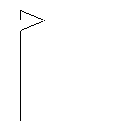
\includegraphics[width=3cm]{pics/fillpolygonsquare1.png}& 
\includegraphics[width=3cm]{pics/fillpolygonsquare2.png}& 
\includegraphics[width=3cm]{pics/fillpolygonsquare3.png}& 
\includegraphics[width=3cm]{pics/fillpolygonsquare4.png}\\ 
Step 1& Step 2& Step 3& Step 4\\
\end{tabular}
\end{center}
\item A second example that draws a five pointed star:
\begin{verbatim}
repeat 5 [forward 100 fillpolygon [back 100 right 144 forward 100 ] back 100 left 72]
\end{verbatim}
\begin{center}
 \begin{tabular}{ccccc}
 
\includegraphics[width=3cm]{pics/fillpolygon1.png}& 
\includegraphics[width=3cm]{pics/fillpolygon2.png}& 
\includegraphics[width=3cm]{pics/fillpolygon3.png}& 
\includegraphics[width=3cm]{pics/fillpolygon4.png}& 
\includegraphics[width=3cm]{pics/fillpolygon5.png}\\
Step 1& Step 2& Step 3& Step 4&Step 5\\
\end{tabular}
\end{center}
\end{itemize}
\section{Break commands}
\xlogo\ has three break commands: \texttt{stop}, \texttt{stopall} and \texttt{op, output}.\\
\prim{stop}{}
\texttt{stop} can have two results. 
\begin{itemize}
 \item If it is included in a \texttt{repeat} or \texttt{while} loop, the program jumps out of the loop there and then.
 \item  If it occurs in a procedure, the program breaks out of the procedure immediately.
\end{itemize}
\noindent \prim{stopall}{} 
The program breaks out of all procedures immediately and stops.\\
\prim{output, op}{} 
\texttt{output, op} allows breaking out of a procedure with a value to be returned.
\section{Multiturtle Mode}
It's possible to have several active turtles on the screen. By default, on Xlogo startup, only one turtle is available. Its number is 0. If you want to "create" a new turtle, you can use the primitive \texttt{setturtle} followed by the number of the turtle. To prevent obstruction, the turtle is created on the origin and is invisible (you must use \texttt{showturtle} to show it). Then, the new turtle is the active turtle, it obeys all classic primitives while you don't change the active turtle with \texttt{setturtle}. The maximum number of available turtles can be set in menu Options - Preferences - Tab options.\\
\\
Here are the primitives for the multiturtle mode:\\
\prim{setturtle, sturtle}{n}
The turtle numero $n$ is now the active turtle. By default on Xlogo startup the active turtle is the number 0.\\
\prim{turtle}{}
Returns the number of the active turtle. \\
\prim{turtles}{}
Returns a list which contains all the numero af the turtles actually on the screen. \\
\prim{eraseturtle, ert}{n}
Delete the turtle number $n$\\
\prim{setTM, setturtlesmax}{n}
Set the maximum number of turtles for multiturtle mode.\\
\prim{tm, turtlesmax}{}
Returns the maximum number of turtles for multiturtle mode.
\section{Play music}
\subsection{Playing music using MIDI synthetizer}
\noindent 
\prim{sequence, seq}{list}
Put in memory the sequence in the list. Read after this table how to write a sequence.\\
\prim{play}{}
Play the sequence in memory. \\
\prim{instrument, instr}{}
Returns the number that corresponds to the selected instrument.  \\
\prim{setinstrument, sinstr}{n}
The selected instrument is now the instrument number $n$. You can see the list of all available instruments in menu Options-Preferences-Tab Sound.\\
\prim{indexsequence, indseq}{}
Returns where the cursor is located in the current sequence.\\
\prim{setindexsequence, sindseq}{n}
Put the cursor to index $n$ in the current sequence in memory.\\
\prim{deletesequence, delseq}{}
Delete the current sequence in memory. \\ \\ 
If you want to play music, you must put the notes in memory in a list called sequence. To create the sequence, you can use the primitive \texttt{seq} or \texttt{sequence}.\\ \\
 These are the rules to follow to create a valid sequence:\\
\texttt{do re mi fa sol la si} : the usual notes of the first octave.\\
To make a sharp re, we note \texttt{re +}\\
To make a flat re, we note \texttt{re -}\\
If you want to go up or down and octave, we use symbol ":" followed by + or -. E.g. After :++ in the sequence, all the notes will be played two octaves up (two ++)
. \\
By default, notes are played for a duration of one. If you want to increase or decrease, you write the number that corresponds to the duration of notes. E.g. \texttt{seq [sol 0.5 la si]}. will play sol with a duration 1 and la si with a duration 0.5 (twic as fast).\\
If you want to play this example:\\
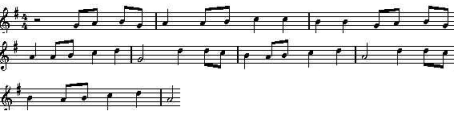
\includegraphics{pics/partition.png}
\begin{verbatim}
to tabac
# create the sequence of notes
seq [0.5 sol la si sol 1 la 0.5 la si 1 :+ do do :- si si 0.5 sol la si sol
          1 la 0.5 la si 1 :+ do re 2 :- sol ]
seq [:+ 1 re 0.5 re do 1 :- si 0.5 la si 1 :+ do re 2 :- la ]
seq [:+ 1 re 0.5 re do 1 :- si 0.5 la si 1 :+ do re 2 :- la ]
seq [0.5 sol la si sol 1 la 0.5 la si 1 :+ do do :- si si 0.5 sol la si sol
          1 la 0.5 la si 1 :+ do re 2 :- sol ]
end
\end{verbatim}

To hear music, launch the command: \texttt{tabac play}\\
Now, we can see/hear an interesting application of the primitive {sindseq}. Write those commands:\\

\begin{verbatim}
delseq       # Delete the sequence in memory
tabac       # Put in memory the notes
sindseq 2   # Put the cursor on the second "la".
tabac       # Put in memory the same sequence but translated of 2.
play        # Great!
\end{verbatim}

You can choose your instrument with the primitive \texttt{sinstr} or with the menu Options-Preferences-Tab sound. You will find the list of all available instruments with their associated number.
\subsection{Playing MP3}
\noindent\prim{mp3play}{word1}
Reads the mp3 file \textit{word1}. This file has to be located in the current folder, you can access a network path too. Here are some examples:\\
\texttt{mp3play file.mp3}\\
\texttt{mp3play http://website.com/file.mp3}\\
\prim{mp3stop}{}
Stops to play the current mp3 file.
\section{Loops:}
XLOGO has seven primitives which allow the construction of loops: \texttt{repeat}, \texttt{for} , \texttt{while}, \texttt{foreach}, \texttt{forever}, \texttt{repeatwhile} and \texttt{repeatuntil}.
\subsection{A loop with \texttt{repeat}}
\noindent \prim{repeat}{n list\_of\_commands} 
\textit{n} is a whole number and \texttt{list\_of\_commands} is a
list containing the commands to execute. The LOGO interpreter will
implement the commands in the list n times: that avoids the need to
copy the same command n times!\\
 Eg: \begin{verbatim}
repeat 4 [forward 100 left 90]      # A square of side 100
repeat 6 [forward 100 left 60]      # A hexagon of side 100
repeat 360 [forward 2 left 1]       # A uh... 360-gon of side 2
                                           # In short, almost a circle!
\end{verbatim}
\noindent
\prim{repcount}{}
Included in a \texttt{repeat} loop. Its an internal variable. Returns the number of the running iteration. (The first iteration is number 1).

\begin{verbatim}
repeat 3 [pr repcount]
1
2
3
\end{verbatim}
\subsection{A loop with \texttt{for}}
\noindent \prim{for}{list1 list2}
\texttt{for} assigns to a variable some successive values in a fixed range with a choosen increment.\\
\textit{list1} contains three arguments: the variable name, the start value, the end value.\\
A fourth argument is optionnal representing the increment (the step between two successive values). Default value is 1. Here are a few examples:
\begin{verbatim}
for [i 1 4][pr :i*2]
2
4
6
8

# Now, i is going from 7 to 2 falling down of 1.5 each times
# Look at the negative increment
# Then, Displays its square.

for [i 7 2 -1.5 ][pr list :i power :i 2]
 
7 49
5.5 30.25
4 16
2.5 6.25
\end{verbatim}
\subsection{A loop with \texttt{while}}
\noindent \prim{while}{list\_to\_evaluate list\_of\_commands}
\textit{list\_to\_evaluate} is a list containing an instruction set
which can be evaluated as a boolean. \textit{list\_of\_commands} is
a list containing the commands to execute. The LOGO interpreter will
continue implementing the \textit{list\_of\_commands} so long as the
\textit{list\_to\_evaluate} is returned as true.\\
 Eg: \begin{verbatim}

while ["true] [rt 1]                    # The turtle will turn around

# An example which allows us to spell the alphabet in reverse

make "list "abcdefghijklmnopqrstuvwxyz
while [not empty? :list] [pr last :list make "list butlast :list]
\end{verbatim}
\subsection{A loop with \texttt{foreach}}
\noindent \prim{foreach}{variable\_name arg1 instructions}
The variable has for successive value the item from a list, or the character from a word. The instructions are repeated for each value of the variable.
\begin{verbatim}
foreach "i "XLOGO [print :i]
X
L
O
G
O
foreach "i [a b c] [print :i]
a
b
c

make "sum 0 foreach "i 12345 [make "sum :sum+:i] print :sum
15
\end{verbatim}

\subsection{A loop with \texttt{forever}}
\noindent \prim{forever}{instructions\_list}
Repeats forever a block of instructions waiting for a command to stop the loop. \\
\begin{verbatim}
Eg: forever [fd 1 rt 1]
\end{verbatim}
\textbf{Be careful when you use this primitive because of the infinite loop!}\\
\subsection{A loop with \texttt{repetewhile}}
\noindent \prim{repeatwhile dowhile}{list1 list2}
Repeats a block of instructions contained in \textit{list1} while \textit{list2} is true.\\
The main difference with the primitive \texttt{while} is that the bloack of instructions is at least executed one times even if \textit{list2} is false.
\begin{verbatim}
make "i 0
repeatwhile [pr :i make "i :i+1] [:i<4]
0
1
2
3
4
\end{verbatim}
\subsection{A loop with \texttt{repeatuntil}}
\noindent \prim{repeatuntil dountil}{list1 list2}
Repeats a block of instructions contained in \textit{list1} until \textit{list2} will be true.
\begin{verbatim}
make "i 0
repeatuntil [pr :i make "i :i+1] [:i>4]
0
1
2
3
4
\end{verbatim}
\section{Receiving input from the user }
%At the moment, XLOGO can interact with the user during the execution
%of a program through the keyboard and through the mouse.
\subsection{Interact with the keyboard}
Currently, text can be accepted from the user during program execution mainly
via 3 primitives: \texttt{key?}, \texttt{readchar} and \texttt{read}.\\ \\
\prim{key?}{}
Is read as true or false according to whether a key has been pressed or not since the start of program execution.\\
\prim{readchar}{}
\begin{itemize}
\item If \texttt{key?} is false, the program is paused until the user presses a key. 
\item If \texttt{key?} is true, it gives the key which was pressed last.
\end{itemize}
These are the values given for particular keys:\\
\begin{table}[h]
\begin{tabular}{|lllll|}
\hline
A ---> 65 & B ---> 66 & C ---> 67 & etc ... & Z ---> 90\\
$\leftarrow$ ---> -37 or -226 (NumPad) & $\uparrow$ ---> -38 or -224  & $\rightarrow$ ---> -39 or -227  & $\downarrow$ ---> -40 or -225 &\\
Echap ---> 27 & F1 ---> -112 & F2 ---> -113 & .... & F12 ---> -123\\
Shift ---> -16 & Espace ---> 32 & Ctrl ---> -17 & Enter ---> 10 &\\
\hline
\end{tabular}
\caption{Values for particular keys}
\end{table}
If you are uncertain about the value returned by a key, you can type:\\
 \texttt{pr readchar}. The interpreter will then wait for you to type
on a key before giving you the corresponding value.\\
\\
\prim{read}{list1 word2}
Presents a dialogue box whose title is \textit{list1}. The user can then input a response in a text field, and the response will be stored in the form of a word or a list (if the user wrote several words) in the variable \textit{word2}, and will be evaluated when the OK button is pressed.

\subsection{Some examples of usage:}

\begin{verbatim}
to vintage
read [What is your age?] "age
make "age :age
if :age<18 [pr [you are a minor]]
if or :age=18 :age>18 [pr [you are an adult]]
if :age>99 [pr [Respect is due!!]]
end

to rallye
if key? [
	make "car readchar
	if :car=-37 [lt 90]
	if :car=-39 [rt 90]
	if :car=-38 [fd 10]
	if :car=-40 [bk 10]
	if :car=27 [stop]
]
rallye
end
# You can control the turtle with the keyboard, and stop with Esc

\end{verbatim}
\subsection{Interact with the mouse}
Currently, mouse events can be accepted from the user during program execution via three primitives: \texttt{readmouse}, \texttt{mousepos} and \texttt{mouse?}. \\ \\
\prim{readmouse}{}
The program is paused until the user presses the mouse. Then, it returns a number that represents the event. These are the differents values:
\begin{itemize}
 \item 0$\to$The mouse has moved.
 \item 1$\to$The button 1 has been pressed.
 \item 2$\to$The button 2 has been pressed.
\end{itemize}
The button 1 is the left button , the button 2 is the next on the right ...\\
\prim{mousepos, mouseposition}{}
Returns a list that contains the position of the mouse.\\
\prim{mouse?}{}
Returns \texttt{true} if we touch the mouse since the program begins. Returns \texttt{false} otherwise.
\subsection{Some examples of usage:}
In this first procedure, the turtle follows the mouse when it moves on the screen.
\begin{verbatim}
to example
# when the mouse moves, go to the next position
if readmouse=0 [setpos mousepos]
example
end
\end{verbatim}
In this second procedure, it's the same but you must click with the left button of the mouse if you want the turtle to move.

\begin{verbatim}
to example2
if readmouse=1 [setpos mousepos]
example2
end
\end{verbatim}
In this third example, we create two pink buttons. If we left-click on the left button, we draw a square with a side of 40. if we left-click on the right button, we draw a little circle. Last, if we right-click on the right button, it stops the program.

\includegraphics*[width=15 cm]{pics/lissouris.png}
\begin{verbatim}
to button
#create a pink rectangular button (height 50 - width 100) 
repeat 2[fd 50 rt 90 fd 100 rt 90] 
rt 45 pu fd 10 pd setpc [255 153 153]
fill bk 10 lt 45 pd setpc 0
end

to lance
cs button pu setpos [150 0] pd button
pu setpos [30 20] pd label "Square
pu setpos [180 20] pd label "Circle
pu setpos [0 -100] pd
mouse
end

to mouse
# we put the value of readmouse in the variable ev
make "ev readmouse
# we put the first coordinate of the mouse in variable x
make "x item 1 mousepos
# we put the second coordinate of the mouse in variable y
make "y item 2 mousepos
# When we click on the left button
if :ev=1 & :x>0 & :x<100 & :y>0 & :y<50 [square]
# When we click on the right button
if  :x>150 & :x<250 & :y>0 & :y<50 [
          if :ev=1 [circle]
          if :ev=3 [stop]
]
mouse
end

to circle
repeat 90 [fd 1 lt 4] lt 90 pu  fd 40 rt 90 pd
end

to square
repeat 4 [fd 40 rt 90] rt 90 fd 40 lt 90
end
\end{verbatim} 
\subsection{Graphical components}
With XLogo, you can add several graphical components on the drawing area (Button or Menu). All the primitives allowing the user to manipulate those components start with  the prefix  \textsc{gui} (for Graphical User Interface).
\subsubsection{Create a component}
First, you need to create those graphical objects, then you can modify some of their properties and last, you can display them on the drawing area
\begin{itemize}
 \item To create a button:\\
\prim{guibutton}{word1 word2}
Create a button whose title is \textit{word2}. The button name is \textit{word1} \\
 \item To create a combo Menu:\\
\prim{guimenu}{word1 list2}
This command creates a combo menu which name is \textit{word1} and which contains items from \textit{list2}\\
\texttt{guimenu "myMenu [item1 item2 item3]}
\end{itemize}
\subsubsection{Modify some properties of graphical components}
\noindent \prim{guiposition}{word1 list2} 
Locates the graphical element \textit{word1} on a specific place with its coordinate. For example, if you want to put the button at the point with coordinates $(20;100)$, you will write:\\
\begin{verbatim}
 guiposition "b [20 100]
\end{verbatim}
If you don't specify a location for the component, it will be placed by default on the upper left corner of the drawing area.\\
\prim{guiremove}{word1}
Remove a graphical component. For example, to delete the button:
\begin{verbatim}
 guiremove "b
\end{verbatim}
\noindent \prim{guiaction}{word1 list2}
Defines an action for the component when the user interacts with it.\\
\begin{verbatim}
# the turtle forwards of 100 if we click on the button "b
 guiaction "b [fd 100 ]

# For the combo menu, each  item has its own action
guiaction "m [[print "item1]  [print "item2] [print "item3]]
\end{verbatim}
\noindent \prim{guidraw}{word1}
Displays the graphical component on the drawing area. For example, to display the button:\\
\begin{verbatim}
 guidraw "b
\end{verbatim}
\section{Time and date}
\xlogo\ has several primitives for date, time or generating countdown.\\
\prim{wait}{n}
 Halts the program, and therefore the turtle, for $\frac{n}{60}$ seconds.  \\
\prim{countdown}{n}
Starts a countdown of $n$ seconds. We know if this countdown has finished with the primitive \texttt{endcountdown?}\\
\prim{endcountdown?}{}
Returns \texttt{"true} if there's no active countdown. Returns \texttt{"false} if the countdown is active.\\
\prim{date}{}
Returns a list wich contains three integers representing the date. The first integer indicates the day, the second the month and the last the year. ---> [day month year]\\
\prim{time}{}
Returns a list of three integers representing the time. The first integer indicates the hour, the second the minutes and the last the seconds. ---> [hour minute seconde]\\
\prim{pasttime}{}
 Returns the past time in seconds since \xlogo has started.\\ \\
Difference between \texttt{wait} and \texttt{countdown} is that \texttt{countdown} doesn't halt the program.\\ \\
Here is an example:
\begin{verbatim}
to clock
# shows time in numerical format
# we refresh the time each five seconds
if endcountdown? [
cs 
sfont 75 ht
make "heu time
make "h first :heu
make "m item 2 :heu
# We shows two number for seconds and minutes. (we must add a 0)
if :m-10<0 [make "m word 0 :m]
make "s last :heu
# We shows two number for seconds and minutes. (we must add a 0)
if :s-10<0 [make "s word 0 :s]
label word word word word :h ": :m ": :s 
countdown 5
]
clock
end
\end{verbatim} 

\section{Using a network with XLogo}
\label{network}
\subsection{The network How to}
First, we have to introduce the basis for network communication before we can use the \xlogo\ primitives.
\begin{figure}[h]
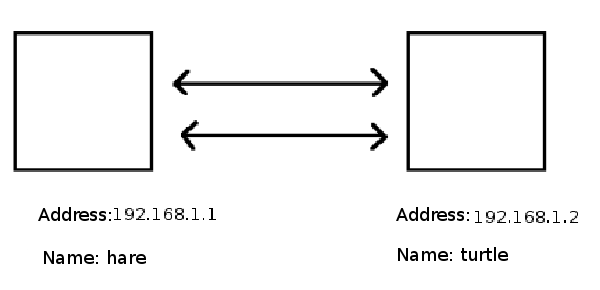
\includegraphics{pics/network.png}
\caption{A simple network}
\end{figure}
Two computers (or more) can communicate through a network if they both have ethernet cards. Each computer is identified by a personal address called an \textit{IP~address}. This IP address consists of four integers, each between 0 and 255 and separated by a dot. For example, The IP address of the first computer in the illustration is 192.168.1.1\\ \\
Because it's not easy to remember these numbers, it's also possible to identify each computer by a more usual name. As can be seen in the illustration, we can communicate to the right computer with its IP address: 192.168.1.2, or with its name: \texttt{turtle}\\ \\
For the moment, I'll add just one more thing. The local computer on which you are working is located by the address: 127.0.0.1. Its general name is \texttt{localhost}. We will see this later in practice. 
\subsection{Primitives for networking} 
\xlogo\ has 4 primitives that allow it to communicate over a network: \texttt{listentcp}, \texttt{executetcp}, \texttt{chattcp} and \texttt{send}. In all future examples, we will take the case of the two computers in the previous figure.
\prim{listentcp}{}
This primitive \texttt{listentcp} is the basis for all network communication. It doesn't need an argument. When you execute this primitive on a computer, the computer will listen for instructions sent from other computers on the network. \\
\prim{executetcp}{word1 list2}
 this primitive allows execution of instructions by a computer on the network.\\
\textit{word1} is the called IP address or computer name, the \textit{list2} contains instructions to execute.\\ \\
Example: I'm on computer \texttt{hare}, I want to draw a square with a side of 100 on the other computer.  Thus, on the computer  \texttt{turtle}, I have to launch the command \texttt{listentcp}. Then, on the computer \texttt{hare}, I write:\\
\begin{verbatim}
 executetcp "192.168.1.2 [repeat 4[fd 100 rt 90]]
or 
 executetcp "turtle [repeat 4[fd 100 rt 90]]
\end{verbatim}
\noindent \prim{chattcp}{word1 list2}
Allows chat between two computers on a network. On each computer, it displays a chat window.\\
\textit{word1} is the called IP address or computer name, \textit{list2} contains the sentence to display.\\ \\
Example: \texttt{hare} wants to talk with \texttt{turtle}.\\
First \texttt{turtle} executes \texttt{listentcp} so it is waiting for instructions from network computers. Then \texttt{hare} writes: \texttt{chattcp~"192.168.1.2~[hello turtle]}.\\
Chat windows will open on both computers, allowing them to talk with each other.\\ 
\prim{sendtcp}{word1 list2}
Send data towards a computer on the network and return his answer.\\ \\
\textit{word1} is the called IP address or computer name, \textit{list2} contains the data to send. When Xlogo is launched on the other computer, il will answer OK. It is possible with this primitive to communicate with a robot through its network interface. Then, the answer of the robot could be different.\\ \\
Example: \texttt{turtle} wants to send to \texttt{hare} the sentence "3.14159 is quite pi".\\
First \texttt{hare} executes \texttt{listentcp} so it is waiting for the other computer to communicate. Then, \texttt{turtle} writes: \texttt{print~sendtcp~"hare~[3.14159 is quite pi]}.\\ \\
\textbf{A little hint}: Launch two instances of \xlogo\ on the same computer.
\begin{itemize}
 \item In the first window, execute \texttt{listentcp}.
 \item In the second one, write \texttt{executetcp "127.0.0.1 [fd 100 rt 90]}
\end{itemize}
You can move the turtle in the other window! (heh, heh, it's possible because 127.0.0.1 designates your local address, so it's your own computer...)




